%------------------------------------------------------------------------------
% Based on https://www.overleaf.com/latex/templates/charless-cv-template/mnhkbhwyytfv
%------------------------------------------------------------------------------
\documentclass[A4,10pt]{article}
\usepackage{latexsym}
\usepackage[]{fullpage}
\usepackage{titlesec}
\usepackage{marvosym}
\usepackage[usenames,dvipsnames]{color}
\usepackage{verbatim}
\usepackage{enumitem}
\usepackage[hidelinks]{hyperref}
\usepackage[english]{babel}
\usepackage{tabularx}
\usepackage{tikz}
\usepackage{fontawesome}
\usepackage{orcidlink}
\usepackage{fancyhdr}
\usepackage{lastpage}
\usepackage[nodayofweek,level]{datetime}
\input{glyphtounicode}
\pagestyle{fancy}
\fancyhf{} % sets both header and footer to nothing
\renewcommand{\headrulewidth}{0pt}

\usepackage[margin=1in, includeheadfoot]{geometry}

\rhead{\color{gray}\thepage \hspace{1pt}(\pageref{LastPage})}
\fancyhead[L]{\color{gray} \today}
%-----FONT OPTIONS-------------------------------------------------------------

% serif
\usepackage{palatino}
% \usepackage{times} %This is the default as well
% \usepackage{charter}

% sans-serif
% \usepackage{helvet}
% \usepackage[sfdefault]{noto-sans}
% \usepackage[default]{sourcesanspro}

%-----PAGE SETUP---------------------------------------------------------------

% Adjust margins
\addtolength{\oddsidemargin}{-0.5cm}
\addtolength{\evensidemargin}{-0.5cm}
\addtolength{\textwidth}{1cm}
\addtolength{\topmargin}{-3cm}
\addtolength{\textheight}{2cm}
\addtolength{\headwidth}{2cm}
\addtolength{\headheight}{2cm}

\urlstyle{same}

\raggedbottom
\raggedright
\setlength{\tabcolsep}{0cm}

% Sections formatting
\titleformat{\section}{
	\vspace{-4pt}\scshape\raggedright\large
}{}{0em}{}[\color{black}\titlerule \vspace{-5pt}]

% Ensure that .pdf is machine readable/ATS parsable
\pdfgentounicode=1

%-----CUSTOM COMMANDS FOR FORMATTING SECTIONS----------------------------------
\newcommand{\CVItem}[1]{
	\item\small{
		{#1 \vspace{-2pt}}
	}
}

\newcommand{\CVSubheading}[4]{
	\vspace{-2pt}\item
	\begin{tabular*}{0.97\textwidth}[t]{l@{\extracolsep{\fill}}r}
		\textbf{#1} & #2 \\
		\small#3 & \small #4 \\
	\end{tabular*}\vspace{-7pt}
}

\newcommand{\CVSubSubheading}[2]{
	\item
	\begin{tabular*}{0.97\textwidth}{l@{\extracolsep{\fill}}r}
		\text{\small#1} & \text{\small #2} \\
	\end{tabular*}\vspace{-7pt}
}

\newcommand{\CVSubItem}[1]{\CVItem{#1}\vspace{-4pt}}

\renewcommand\labelitemii{$\vcenter{\hbox{\tiny$\bullet$}}$}

\newcommand{\CVSubHeadingListStart}{\begin{itemize}[leftmargin=0.5cm, label={}]}
\newcommand{\CVSubHeadingListEnd}{\end{itemize}}
\newcommand{\CVItemListStart}{\begin{itemize}}
\newcommand{\CVItemListEnd}{\end{itemize}\vspace{-5pt}}

%------------------------------------------------------------------------------
% CV STARTS HERE  %
%------------------------------------------------------------------------------

\begin{document}
	
	\begin{minipage}[c]{0.05\textwidth}
		\-\
	\end{minipage}
	\begin{minipage}[c]{0.225\textwidth}
		\begin{tikzpicture}
			\clip (0,0) circle (1.75cm);
			\node at (0,0) {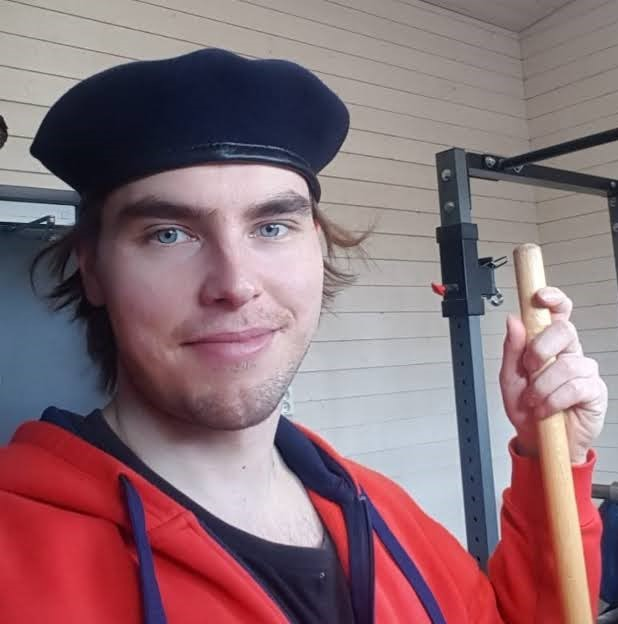
\includegraphics[width = 3.5cm]{portrait.jpg}}; 
		\end{tikzpicture}
		\hfill\vline\hfill
	\end{minipage}
	\begin{minipage}[c]{0.5\textwidth}
		\textbf{\Huge \scshape{Tuomas Borman}} \\ \vspace{1pt} 
		\small{Data Scientist \& Bioinformatician | MSc (Tech) \& MSc (Econ)} \\ \par
		\faPhone \quad +358 40 522 5386 \\
		\href{mailto:tuomas.v.borman@utu.fi}{\faEnvelope \quad tuomas.v.borman@utu.fi} \\
		\href{https://www.linkedin.com/in/TuomasBorman/}{\faLinkedin \quad TuomasBorman} \\
		\href{https://github.com/TuomasBorman}{\faGithub \quad TuomasBorman} \\
		\href{https://orcid.org/0000-0002-8563-8884}{\orcidlink{} \quad 0000-0002-8563-8884}
	\end{minipage}
	
	\section{Work Experience}
	\CVSubHeadingListStart
	\CVSubheading
	{Doctoral Researcher (Data Science)}{January 2023 -- Present}
	{University of Turku}{Turku, Finland}
	
	\CVSubheading
	{Project Worker}{April 2022 -- Present}
	{Handata Oy}{Turku, Finland}
	\CVItemListStart
	\CVItem{Developed business intelligence tools.}
	\CVItemListEnd
	
	\CVSubheading
	{Project Researcher (Data Science)}{July 2022 -- December 2022}
	{University of Turku}{Turku, Finland}
	\CVItemListStart
	\CVItem{Analyzed biomedical data and developed data science tools.}
	\CVItemListEnd
	
	\CVSubheading
	{Research Assistant (Data Science)}{October 2020 -- July 2022}
	{University of Turku}{Turku, Finland}
	\CVItemListStart
	\CVItem{Analyzed biomedical data and developed data science tools.}
	\CVItemListEnd
	
	\CVSubheading
	{Teaching Assistant (Biotechnology)}{Oct 2020 -- Nov 2020 \& Jan 2021 -- Feb 2021}
	{University of Turku}{Turku, Finland}
	\CVItemListStart
	\CVItem{Teaching on a M.Sc level laboratory course (Laboratory Exercises in Molecular Biotechnology).}
	\CVItem{Teaching on a B.Sc level laboratory course (Biotechnical Systems).}
	\CVItemListEnd
	\CVSubHeadingListEnd
	
	\section{Education}
	\CVSubHeadingListStart
	\CVSubheading
	{{Doctor of Science (Technology) $|$ \emph{\small{Information and Communication Technology}}}}{2023 -- (2026)}
	{University of Turku}{Turku, Finland}
	
	\CVSubheading
	{{Master of Science (Economics and Business Administration) $|$ \emph{\small{Accounting and Finance}}}}{2022 -- 2023}
	{University of Turku}{Turku, Finland}
	
	\CVSubheading
	{{Master of Science (Technology) $|$ \emph{\small{Biotechnology}}}}{2020 -- 2022}
	{University of Turku}{Turku, Finland}
	
	\CVSubheading
	{{Bachelor of Science (Economics and Business Administration) $|$ \emph{\small{Accounting and Finance}}}}{2020 -- 2022}
	{University of Turku}{Turku, Finland}
	
	\CVSubheading
	{{Bachelor of Science (Technology) $|$ \emph{\small{Biotechnology}}}}{2017 -- 2020}
	{University of Turku}{Turku, Finland}
	\CVSubHeadingListEnd
	
	\section{Projects}
	\CVSubHeadingListStart
	\CVSubheading
	{\emph{miaverse} $|$ \emph{\small{R/Bioconductor framework for microbiome analysis}}}{2020 -- Present}
	{\href{https://microbiome.github.io/}{https://microbiome.github.io/}}{}
	\CVItemListStart
	\CVItem{One of the developers of \emph{miaverse}.}
	\CVItem{Maintainer of packages \emph{\href{https://www.bioconductor.org/packages/release/bioc/html/mia.html}{mia}} and \emph{\href{https://www.bioconductor.org/packages/release/bioc/html/miaViz.html}{miaViz}}.}
	\CVItemListEnd
	\CVSubHeadingListEnd
	
	\section{Certificates}
	\CVSubHeadingListStart
	\CVSubheading
	{\href{https://emea-interface.ungerboeck.com/clients/EMBL/Prod/LinkedInCertificates/cert/147764_6070.pdf}{EMBO | EMBL Symposium $|$ \emph{\small{Multiomics to Mechanisms: Challenges in Data Integration}}}}{September 2021}
	{European Molecular Biology Laboratory}{}
	\CVSubheading
	{PMAF Project Management Foundation Certificate $|$ \emph{\small{(IPMA D)}}}{April 2018}
	{Projektiammattilaiset PRY, Project Professionals Finland}{}
	\CVSubHeadingListEnd

	\section{Skills and Interests}
	\begin{itemize}[leftmargin=0.5cm, label={}]
		\small{\item{
				\textbf{Tools and technologies}{: R, Python, SQL, GIT, Statistical Modeling, Machine Learning, Data Mining...} \\
				\textbf{Languages}{: English (Full professional proficiency), Finnish (Native), Swedish (Limited working proficiency), German (Elementary proficiency)} \\		
		}}
	\end{itemize}

\end{document}
